%%%%%%%% ICIIT 2027 submission (ACM sigconf) %%%%%%%%%%%%%%%%%%%%%%%%%%%%%%%%%%%%%%
% Build:  latexmk -pdf main.tex   (needs acmart >= 2.x from TeX Live/CTAN; the
%         acmart.cls v1.90 in the ICIIT zip clashes with current hyperxmp)
% Limit:  5 two-column pages including references (ICIIT; extra pages are charged).
%%%%%%%%%%%%%%%%%%%%%%%%%%%%%%%%%%%%%%%%%%%%%%%%%%%%%%%%%%%%%%%%%%%%%%%%%%%%%%%%

\documentclass[sigconf]{acmart}

\usepackage{multirow}
\usepackage{mathtools}
\usepackage[capitalize,noabbrev]{cleveref}

\usepackage{tikz}
\usetikzlibrary{arrows.meta,positioning,calc,shapes.geometric}
\usepackage{pgfplots}
\pgfplotsset{compat=1.18}
\usepgfplotslibrary{groupplots}

% Shared macros and plot styles.
\newcommand{\usdc}{USDC}
\definecolor{cSRCLA}{HTML}{1F6FD6}
\definecolor{cB0}{HTML}{3C3C3C}
\definecolor{cB1}{HTML}{E8603C}
\definecolor{cB2}{HTML}{1BAF7A}
\definecolor{cB2u}{HTML}{8C8C8C}
\definecolor{cB3}{HTML}{F0A500}
\definecolor{cB4}{HTML}{E46F9A}
\definecolor{cB5}{HTML}{7B52D3}
\pgfplotsset{
  sweep/.style={
    xmode=log, log basis x=10,
    width=\linewidth, height=5.2cm,
    xmin=8000, xmax=12500000,
    xtick={1e4,1e5,1e6,1e7},
    xticklabels={10k,100k,1M,10M},
    xlabel={Pool size (USDC, log scale)},
    tick label style={font=\scriptsize},
    label style={font=\footnotesize},
    grid=major, grid style={gray!20},
    every axis plot/.append style={line width=0.8pt, mark size=1.3pt},
    legend style={font=\scriptsize, draw=none, fill=none, legend columns=4,
                  column sep=4pt},
    unbounded coords=jump,
  },
  pSRCLA/.style={cSRCLA, mark=*, line width=1.4pt},
  pB0/.style={cB0, densely dotted, mark=square},
  pB1/.style={cB1, dashed, mark=square*},
  pB2/.style={cB2, mark=triangle*},
  pB2u/.style={cB2u, dashed, mark=o},
  pB3/.style={cB3, dashed, mark=diamond*},
  pB4/.style={cB4, mark=triangle*, mark options={rotate=180}},
  pB5/.style={cB5, dashdotted, mark=diamond},
}
% \sweepplots{<data file>}: the eight policies of the thesis sweep figures.
\newcommand{\sweepplots}[1]{%
  \addplot[pSRCLA] table[x=tier,y=srcla]{#1};
  \addplot[pB0]    table[x=tier,y=b0]{#1};
  \addplot[pB1]    table[x=tier,y=b1]{#1};
  \addplot[pB2]    table[x=tier,y=b2]{#1};
  \addplot[pB2u]   table[x=tier,y=b2u]{#1};
  \addplot[pB3]    table[x=tier,y=b3]{#1};
  \addplot[pB4]    table[x=tier,y=b4]{#1};
  \addplot[pB5]    table[x=tier,y=b5]{#1};
}
\newcommand{\sweeplegend}{%
  \legend{SRCLA, B0 idle, B1 highest displayed, B2 capacity-aware,
          B2u B2 no reserve, B3 B2 + cost hurdle, B4 frozen equal split, B5 hindsight}}


% Let long URLs in the references break at any character.
\makeatletter\g@addto@macro{\UrlBreaks}{\UrlOrds}\makeatother

% No word splitting across lines; let justified lines stretch instead.
\hyphenpenalty=10000
\exhyphenpenalty=10000
\tolerance=2000
\emergencystretch=2em

%% Submission version. ICIIT's own ACM template has no copyright/permission
%% box, and generates the ACM Reference Format after acceptance. For
%% camera-ready, replace the next two lines with the rights commands ACM sends
%% after the eRights form (\setcopyright{...}, \acmDOI{...}, \acmISBN{...}).
\setcopyright{none}
\settopmatter{printacmref=false}
\renewcommand\footnotetextcopyrightpermission[1]{}
\copyrightyear{2027}
\acmYear{2027}
\acmDOI{}
\acmISBN{}
\acmConference[ICIIT 2027]{2027 12th International Conference on Intelligent Information Technology}{March 4--7, 2027}{Ho Chi Minh City, Vietnam}

\begin{document}

\title[An Optimized Allocation Algorithm for Decentralized Lending Markets]{An Optimized Allocation Algorithm for Pooled Stablecoin Deposits across Decentralized Lending Markets}

% Every author carries both affiliations (supervisor's instruction): UIT and
% VNU-HCM. Authors that share affiliations are grouped as in the ACM sample.
\author{Ngoc Anh Khoa Nguyen}
\email{23520750@gm.uit.edu.vn}
\author{Nguyen Thuy Anh Truong}
\email{23520082@gm.uit.edu.vn}
\author{Toan Tan Nguyen}
\email{toannt@uit.edu.vn}
\affiliation{%
  \institution{University of Information Technology}
  \city{Ho Chi Minh City}
  \country{Vietnam}}
\affiliation{%
  \institution{Vietnam National University Ho Chi Minh City}
  \city{Ho Chi Minh City}
  \country{Vietnam}}

\renewcommand{\shortauthors}{Nguyen et al.}

% Printed author block in the supervisor's format: names with numbered
% affiliation marks, then the numbered affiliations. The \author/\affiliation
% data above still feed the ACM Reference Format and the PDF metadata.
\makeatletter
\def\@mkauthors{\begingroup
  \hsize=\textwidth
  \global\setbox\mktitle@bx=\vbox{\noindent
    \unvbox\mktitle@bx\par\medskip\centering
    {\large Ngoc Anh Khoa Nguyen\textsuperscript{1,2},
      Nguyen Thuy Anh Truong\textsuperscript{1,2},
      Toan Tan Nguyen\textsuperscript{1,2}\par}\smallskip
    {\normalsize
      \textsuperscript{1}University of Information Technology, Ho Chi Minh City, Vietnam\par
      \textsuperscript{2}Vietnam National University Ho Chi Minh City, Ho Chi Minh City, Vietnam\par}\smallskip
    {\small \href{mailto:23520750@gm.uit.edu.vn}{23520750@gm.uit.edu.vn},
      \href{mailto:23520082@gm.uit.edu.vn}{23520082@gm.uit.edu.vn},
      \href{mailto:toannt@uit.edu.vn}{toannt@uit.edu.vn}\par}\bigskip}%
  \endgroup}
\makeatother

\begin{abstract}
Decentralized lending markets hold tens of billions of US dollars, and a growing share of this capital is managed by pooled vaults that spread one stablecoin across several markets. Most of these allocators follow the highest advertised supply rate, although that rate falls once the pool deposits, says nothing about whether a market can still repay its suppliers, and ignores reallocation fees. For a pool that must honor withdrawals at any time, choosing where to lend is therefore a liquidity-risk problem as much as a yield problem. We propose SRCLA (Safe, Robust, Cost-Aware Lending Allocation), an allocation algorithm that helps a pool earn yield across lending markets while always being able to repay its depositors. It screens markets, evaluates rates after the pool's own deposit, maximizes a calibrated lower bound on forecast yield, keeps a stress-sized reserve, and moves capital only when the conservative gain repays the cost. On hourly on-chain data from three USDC markets on the Base blockchain, SRCLA kept the pool withdrawable under every stress scenario at four sizes from $10^4$ to $10^7$~USDC over 86 held-out days and stayed within a 43 basis-point non-inferiority margin in 13 of 14 comparisons, while a second period, in which one market lost all of its cash, shows where this protection ends. These results indicate that the algorithm lets pooled deposits earn competitive yield without giving up their withdrawability.
\end{abstract}


% CCS 2012 concepts, IDs checked against ACM's official taxonomy file.
\begin{CCSXML}
<ccs2012>
 <concept>
  <concept_id>10010405.10003550.10003551</concept_id>
  <concept_desc>Applied computing~Digital cash</concept_desc>
  <concept_significance>500</concept_significance>
 </concept>
 <concept>
  <concept_id>10003752.10003809.10003716</concept_id>
  <concept_desc>Theory of computation~Mathematical optimization</concept_desc>
  <concept_significance>300</concept_significance>
 </concept>
 <concept>
  <concept_id>10002950.10003648.10003688.10003693</concept_id>
  <concept_desc>Mathematics of computing~Time series analysis</concept_desc>
  <concept_significance>100</concept_significance>
 </concept>
</ccs2012>
\end{CCSXML}

\ccsdesc[500]{Applied computing~Digital cash}
\ccsdesc[300]{Theory of computation~Mathematical optimization}
\ccsdesc[100]{Mathematics of computing~Time series analysis}

\keywords{decentralized finance, lending markets, allocation under uncertainty, prediction bounds, transaction costs, liquidity risk}

\maketitle


%%%%%%%%%%%%%%%%%%%%%%%%%%%%%%%%%%%%%%%%%%%%%%%%%%%%%%%%%%%%%%%%%%%%%%%%%%%%%%%%
\section{Introduction}
\label{sec:intro}

Stablecoins have become the working currency of decentralized finance (DeFi). Their circulating supply now exceeds 300 billion USD, about 72 billion of it in USDC \citep{defillamastable}, and the 659 lending protocols tracked by DefiLlama hold more than 52 billion USD of deposits \citep{defillamalending}. Each lending market is a smart contract that lends suppliers' deposits to over-collateralized borrowers at a rate set by the borrowed share \citep{gudgeon2020defi,aaveirm}. As these rates differ across markets and change hourly, a growing layer of applications decides for users where to lend: yield aggregators \citep{cousaert2022sok}, curated vaults \citep{metamorpho,eulerhandbook} and, more recently, autonomous allocation agents \citep{ysselection,zyftreasury,mamohow}.

Most of these allocators rank markets by their advertised supply rate, which is a weak guide for a pool that holds other people's money. The rate falls once the pool's own deposit arrives; a position keeps its book value even when the market has lent out all of its cash and no supplier can leave; and every reallocation pays fees that a small rate difference may never repay. Choosing where to lend is therefore a liquidity-risk problem as much as a yield problem.

We address this problem with SRCLA, an allocation algorithm for pooled stablecoin deposits that helps a vault earn yield across lending markets while always being able to repay its depositors; at every epoch it checks each withdrawability constraint before it compares yield. We evaluate it on the USDC markets of Aave~V3, Compound~III and Moonwell on the Base network, an Ethereum layer-2 blockchain, including a period in which an exploit drained Moonwell's market \citep{moonwellpostmortem}. Our contributions are threefold.
\begin{itemize}
  \item We formulate pooled allocation as a sequential decision problem constrained by withdrawable liquidity rather than accounting value (\cref{sec:problem}).
  \item We propose \textbf{SRCLA} (Safe, Robust, Cost-Aware Lending Allocation), an allocation algorithm that combines screening, post-deposit rates, a calibrated yield bound, a stress-sized reserve and cost hurdles (\cref{sec:method}).
  \item We evaluate SRCLA walk-forward on 21,915 hourly observations against six baselines and eight ablations under criteria fixed in advance, reporting unfavourable results as well (\cref{sec:experiments}).
\end{itemize}
The rest of the paper reviews related work (\cref{sec:related}), presents the approach (\cref{sec:approach}), reports the experiments (\cref{sec:experiments}) and concludes (\cref{sec:conclusion}).

%%%%%%%%%%%%%%%%%%%%%%%%%%%%%%%%%%%%%%%%%%%%%%%%%%%%%%%%%%%%%%%%%%%%%%%%%%%%%%%%
\section{Related Work}
\label{sec:related}

Our work draws on three lines of research: how lending markets set their rates, how deployed systems allocate pooled deposits, and how to decide under forecast uncertainty and transaction costs.

\subsection{Lending Markets and Interest-Rate Models}

Lending protocols set rates by a utilization-dependent rule, typically piecewise linear with a kink beyond which the borrow rate rises steeply to draw cash back \citep{aaveirm,compoundrates,moonwellcurves}. Gudgeon et al.~\citep{gudgeon2020defi} first analysed these models systematically, together with their effect on liquidity and market efficiency. Later studies ask how a protocol \emph{should} set rates: AgileRate~\citep{bastankhah2024agilerate} replaces the static curve with an adaptive controller, and Qu et al.~\citep{qu2025rules} learn rate updates by reinforcement learning on Aave data. Both take the protocol's side of the market.

We take the supplier's side, where the rate rule is given and the question is where to lend. Baude et al. adopt this view to optimize leveraged looping as a convex allocation~\citep{baude2026leveraged} and, closest to our work, to split one lender's budget across markets when the lender's own deposit dilutes the rate, a return that is only piecewise concave under a kinked curve~\citep{baude2026capital}. We share this post-deposit model, but a pool serving many depositors also needs a calibrated yield bound, a stress reserve and a cost hurdle.

\subsection{Pooled Allocators in Practice}

Cousaert et al.~\citep{cousaert2022sok} systematize yield aggregators, which pool deposits in a vault and route them to yield-bearing strategies. We read today's deployed systems against the mechanisms a pooled allocator needs, recording a missing mechanism as \emph{not documented} rather than absent.

\emph{Idle Best Yield} comes closest to our post-deposit evaluation: an off-chain bot maximizes the aggregate rate using each protocol's rate \texttt{nextRate}$(x_i)$ after supplying $x_i$ \citep{idleoverview}, but describes no uncertainty model, stress reserve or cost threshold. \emph{Yearn~V3, MetaMorpho and Euler Earn} instead enforce strategy caps, idle minimums, supply caps or timelocks on chain \citep{yearnvault,metamorpho,eulerhandbook}, but leave the rule that chooses the target to an operator. More recent products present allocation as an \emph{autonomous agent}. Yield Seeker checks withdrawable liquidity and proposes a move only when its benefit covers the cost \citep{ysselection}, and ZyfAI checks rate difference, pool safety, break-even and liquidity \citep{zyftreasury}, yet neither publishes thresholds or formulas. Mamo places USDC wherever the available rate is highest \citep{mamohow}, with no stated rule for a top market that has run out of cash.

\begin{table}[t]
\caption{Mechanisms documented by deployed allocators. Y: documented; P: partly; --: not documented. PD: post-deposit rate; LB: forecast lower bound; Cap: market and group caps; Res.: stress-sized reserve; Cost: cost hurdle; OC: limits enforced on chain.}
\label{tab:systems}
\centering
\small
\setlength{\tabcolsep}{5pt}
\begin{tabular}{lcccccc}
\toprule
System & PD & LB & Cap & Res. & Cost & OC \\
\midrule
Idle Best Yield         & Y  & -- & -- & P  & -- & -- \\
Yearn V3                & -- & -- & P  & P  & -- & Y  \\
MetaMorpho / Euler Earn & -- & -- & P  & -- & -- & Y  \\
Yield Seeker            & -- & -- & P  & -- & P  & P  \\
ZyfAI                   & -- & -- & -- & -- & P  & P  \\
Mamo                    & -- & -- & -- & -- & -- & P  \\
\midrule
\textbf{SRCLA}          & Y  & Y  & Y  & Y  & Y  & Y  \\
\bottomrule
\end{tabular}
\end{table}

As \cref{tab:systems} shows, enforcement layers have matured, yet no documented system states a reproducible algorithm that combines a forecast bound, a stress-sized reserve and a cost hurdle, or evaluates it under criteria fixed in advance. No single ingredient of SRCLA is new; our contribution lies in combining them into one deterministic, auditable algorithm.

\subsection{Decisions under Uncertainty and Costs}

Under proportional costs the optimal policy leaves a no-trade region around the target \citep{constantinides1986}, and with predictable returns it trades only partway toward it \citep{garleanu2013}; both results shape our movement rule. Optimizing a conservative bound rather than a point forecast, our bound is an empirical residual quantile in the spirit of conformal prediction, whose guarantee weakens without exchangeability \citep{barber2023conformal}, so we test its coverage on held-out data with the backtests of Kupiec~\citep{kupiec1995} and Christoffersen~\citep{christoffersen1998}.

%%%%%%%%%%%%%%%%%%%%%%%%%%%%%%%%%%%%%%%%%%%%%%%%%%%%%%%%%%%%%%%%%%%%%%%%%%%%%%%%
\section{Proposed Approach}
\label{sec:approach}

This section first specifies the allocation problem (\cref{sec:problem}) and then presents SRCLA, first as a whole and then stage by stage (\cref{sec:method}).

\subsection{Problem Specification}
\label{sec:problem}

In plain terms, a pooled vault holds the deposits of many users and lends them across several markets. A market pays more or less depending on how much the pool supplies, and returns money only while it still holds cash. As depositors may withdraw at any time, the goal is to earn as much interest as possible while always being able to pay them, which requires getting three things right: \emph{liquidity}, how much of the pool can be withdrawn now; \emph{yield}, what each market will conservatively pay after the pool's own deposit; and \emph{cost}, whether a move earns back what it pays. We formalize the first two below; the decision problem adds the third.

\paragraph{Pool and liquidity.}
The pool holds one stablecoin. At discrete epochs $t$ an allocator splits total assets $A_t$ between an idle balance $I_t$ and positions $P_{i,t}$ in $n$ markets, where market $i$ holds cash $C_{i,t}$ and loans $B_{i,t}$. A decision chooses weights $w_0$ (idle) and $w_i$, or positions $x_i = w_i V$ with $V = A_t$. Yet $A_t = I_t + \sum_i P_{i,t}$ is a claim, not cash; what the pool can pay out in one transaction is its \emph{synchronous liquidity}
\begin{equation}
  Q^{\mathrm{sync}}_t = I_t + \textstyle\sum_{i} \min\bigl(P_{i,t},\, C_{i,t}\bigr),
  \label{eq:qsync}
\end{equation}
since a market can return at most the cash it holds. As $C_{i,t}$ approaches zero, $P_{i,t}$ is unchanged while its exitable part vanishes.

\paragraph{Interest-rate model.}
Most lending markets use a borrow rate that is linear on each side of a kink $U^{*}$ \citep{aaveirm,compoundrates,moonwellcurves}:
\begin{align}
  U &= \frac{B}{C+B}, \qquad U'(d) = \frac{B}{C+d+B}, \label{eq:util}\\
  r_b(U) &= r_0 + s_1 \min(U, U^{*}) + s_2 \max(U - U^{*}, 0), \label{eq:borrow}\\
  r_s(U) &= r_b(U)\, U\, (1 - \rho), \label{eq:supply}
\end{align}
with slopes $s_2 > s_1 \ge 0$ and reserve factor $\rho$. A deposit $d$ adds cash but not loans, moving utilization from $U$ to $U'(d)$, which leads to the following property.

\begin{proposition}
\label{prop:monotone}
If $r_b$ is non-decreasing and non-negative on $[0,1]$, the post-deposit supply rate $d \mapsto r_s(U'(d))$ is non-increasing in $d$, and the slope of $r_s$ in $U$ jumps by ${(1-\rho)\,U^{*}(s_2 - s_1)}$ at the kink.
\end{proposition}
\begin{proof}
$U'(d)$ decreases in $d$ and $r_b(U)\,U\,(1-\rho)$ is a product of non-negative, non-decreasing functions; the jump follows from the product rule.
\end{proof}

Ranking markets by the pre-deposit rate thus overstates their yield, most of all for small markets near the kink.

\paragraph{The decision problem.}
At each epoch the allocator observes every market's state and rate parameters, measured fees and prices, the pool's state, and forecast parameters fitted once on past data and then frozen. It must choose a target $x^{*}$ that maximizes a conservative estimate of post-deposit yield, keeps enough synchronous liquidity to meet withdrawals under stress, and is reached only through moves whose expected gain exceeds their cost. It returns $x^{*}$, the reserve $I^{\mathrm{req}}$ that comes with it, and either a \emph{hold} or a \emph{rebalance} plan that withdraws before it deposits; it must be deterministic and fail closed, holding whenever inputs are missing or stale.

\subsection{The SRCLA Algorithm}
\label{sec:method}

\begin{figure*}[t]
  \centering
  % The six decision stages of SRCLA (thesis Figure 3.1), drawn left to right.
% Coordinates are in millimetres; the figure spans \textwidth (171 mm).
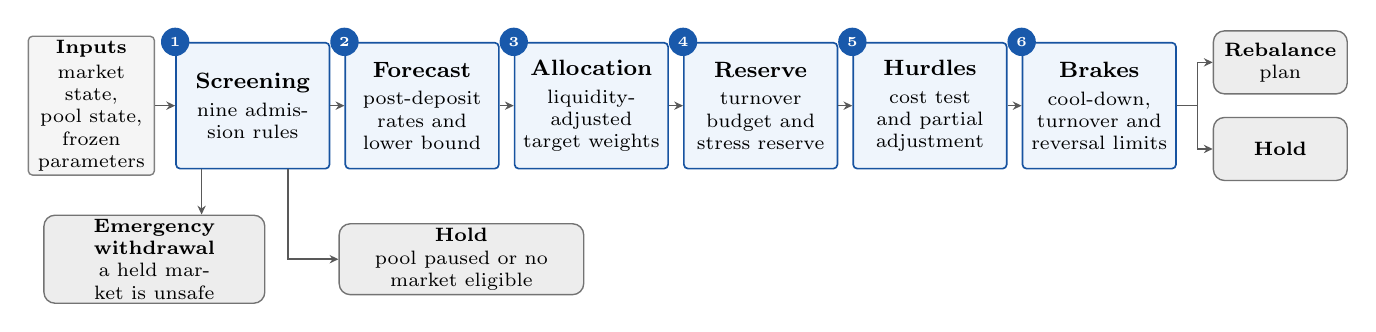
\begin{tikzpicture}[
  x=1mm, y=1mm,
  font=\scriptsize,
  every node/.style={align=center},
  stage/.style={draw=cSRCLA!75!black, fill=cSRCLA!7, rounded corners=1.5pt,
                line width=0.6pt, minimum width=19.5mm, text width=18mm,
                minimum height=16mm, inner sep=1.5pt},
  data/.style={draw=black!50, fill=black!4, rounded corners=1.5pt, line width=0.5pt,
               minimum width=16mm, text width=14.5mm, minimum height=16mm, inner sep=1.5pt},
  outcome/.style={draw=black!55, fill=black!7, rounded corners=4pt, line width=0.5pt,
                  minimum width=17mm, text width=15.5mm, minimum height=8mm, inner sep=1pt},
  early/.style={draw=black!55, fill=black!7, rounded corners=4pt, line width=0.5pt,
                minimum height=9mm, inner sep=1.5pt},
  badge/.style={circle, fill=cSRCLA!80!black, text=white, font=\tiny\bfseries,
                inner sep=0pt, minimum size=3.6mm},
  arr/.style={-{Stealth[length=3.2pt, width=3pt]}, black!65, line width=0.55pt},
  title/.style={font=\footnotesize\bfseries},
]
% input
\node[data] (in) at (8,0) {\textbf{Inputs}\\[1pt] market state, pool state, frozen parameters};

% stages
\foreach \i/\x/\t/\d in {
  1/28.5/Screening/nine admission rules,
  2/50/Forecast/post-deposit rates and lower bound,
  3/71.5/Allocation/liquidity-adjusted target weights,
  4/93/Reserve/turnover budget and stress reserve,
  5/114.5/Hurdles/cost test and partial adjustment,
  6/136/Brakes/{cool-down, turnover and reversal limits}} {
  \node[stage] (s\i) at (\x,0) {{\footnotesize\bfseries \t}\\[2pt] \d};
  \node[badge] at (s\i.north west) {\i};
}

% main flow
\draw[arr] (in) -- (s1);
\foreach \a/\b in {1/2,2/3,3/4,4/5,5/6} \draw[arr] (s\a) -- (s\b);

% final outcomes
\node[outcome] (reb) at (159,5.5) {\textbf{Rebalance}\\ plan};
\node[outcome] (hold) at (159,-5.5) {\textbf{Hold}};
\coordinate (fork) at (148.5,0);
\draw[black!65, line width=0.55pt] (s6.east) -- (fork);
\draw[arr] (fork) |- (reb.west);
\draw[arr] (fork) |- (hold.west);

% early exits from Stage 1
\node[early, text width=27mm] (emg) at (16,-19.5) {\textbf{Emergency withdrawal}\\ a held market is unsafe};
\node[early, text width=30mm] (hold0) at (55,-19.5) {\textbf{Hold}\\ pool paused or no market eligible};
\draw[arr] (s1.south -| 22,0) -- (emg.north -| 22,0);
\draw[arr] (s1.south -| 33,0) |- (hold0.west);
\end{tikzpicture}

  \caption{The six stages of the SRCLA algorithm.}
  \Description{A left-to-right flow of six boxes, screening, forecast, allocation, reserve, hurdles and brakes, ending in a rebalance plan or a hold; screening can branch to an emergency withdrawal or an early hold.}
  \label{fig:stages}
\end{figure*}

To solve this problem, the SRCLA algorithm runs a pipeline of six stages at every epoch (\cref{fig:stages}), from the market and pool state to a hold or a rebalance plan. Two principles run through it: every withdrawability constraint is applied before yield is compared, and any doubt leads to holding. Stage~1 selects the markets that may receive capital, Stage~2 estimates conservatively what each can pay, Stage~3 chooses target weights, Stage~4 limits turnover and sizes the reserve, and Stages~5--6 decide whether moving toward the target is worth its cost.

\paragraph{Stage 1: screening.}
A market may receive capital only if it passes nine rules; for instance, it is not paused, its configuration matches one on record, it has at least 30 observations under its current rate parameters and it is at most 99\% utilized. Only a pause or a configuration change triggers an \emph{emergency withdrawal} of at most 25\% of assets per epoch, and the algorithm then stops; the other rules merely stop new deposits, and if the pool is paused or no market is eligible, the algorithm holds without running the later stages.

\paragraph{Stage 2: post-deposit rates and lower bound.}
For each eligible market we remove the pool's own position from the observed cash and evaluate the supply rate at 16 candidate positions by \eqref{eq:util}--\eqref{eq:supply}. Since yield is realized over a coming horizon $H$, we pair this rate with a one-sided prediction bound. The forecaster is chosen on calibration data alone, mainly by coverage error and breach size; our state-space form forecasts utilization as an exponentially weighted mean with half-life $h$ and maps it through the known rate model, rather than fitting a rate series that jumps at the kink. For market $i$ and position $x$ the bound is relative,
\begin{equation}
  \ell_i(x) = \hat\mu_i(x)\,\bigl(1 + q^{\mathrm{rel}}_i\bigr), \qquad \varepsilon = \frac{y - \hat\mu}{\hat\mu},
  \label{eq:lowerbound}
\end{equation}
where $\hat\mu_i(x)$ is the post-deposit rate over the horizon, $y$ the realized yield and $q^{\mathrm{rel}}_i \in [-1, 0]$ the empirical $p$-quantile of the relative residuals $\varepsilon$ on the calibration period. Were the residuals exchangeable, split-conformal reasoning would give $\Pr[y < \ell] \le p$; realized yields are serially dependent, so coverage is tested on held-out data. Unlike an additive haircut, which turns negative as $\hat\mu_i(x)$ falls with $x$ (\cref{prop:monotone}), the relative bound stays positive.

\paragraph{Stage 3: constrained optimization.}
Given these bounds, the target weights maximize the portfolio lower bound
\begin{equation}
  w^{*} = \arg\max_{w}\ \sum_{i} \varphi_i\, w_i\, \hat\mu_i(w_i V)\,\bigl(1 + q_p(w)\bigr), \quad
  \varphi_i = \frac{\min(x_i, e_i)}{x_i},
  \label{eq:objective}
\end{equation}
where $e_i$ is the market's conservative exit capacity, so capital that cannot leave earns nothing, and $q_p(w)$ is the 1\% quantile of the portfolio's weighted residuals. The constraints are the budget $w_0 + \sum_i w_i = 1$ with $w_0 V \ge I^{\mathrm{req}}(x)$, every stress scenario of Stage~4, a cap per dependency group, and $x_i \le \min(c_i V, \bar{x}_i, \kappa_i, \mathit{liq}_i)$: a percentage cap $c_i$ (50\% here), an absolute cap $\bar{x}_i$, the room $\kappa_i$ under the market's supply cap, and a \emph{structural cap} $\mathit{liq}_i$, the position plus the market's cash, shrinking linearly to zero between 80\% and 100\% utilization. As the objective is not concave \citep{baude2026capital}, we use greedy ascent on a grid of at most 64 steps, verified against exhaustive enumeration; the vault contract also enforces the caps and idle minimum on chain.

\paragraph{Stage 4: turnover budget and reserve.}
The target is first scaled so that one plan moves at most 50\% of assets. The pool must then keep the idle balance
\begin{multline}
  I^{\mathrm{req}}(x) = \max\Bigl\{ I^{\mathrm{floor}},\;
    Q_{\beta}(W_H) - \sum_i \min(x_i, e_i),\\
    \max_s \bigl(D_s - E_s(x)\bigr) \Bigr\},
  \label{eq:reserve}
\end{multline}
the largest of a fixed floor, the $\beta = 0.95$ quantile of withdrawals over the horizon net of immediate exits, and the shortfall over four stress scenarios that demand $D_s$ = 5, 10, 25 and 50\% of assets while cutting exit capacity by $h_s$ = 0, 10, 25 and 50\%, where ${E_s(x) = \sum_i \min\bigl(x_i, (1 - h_s) e_i\bigr)}$. A candidate failing any scenario is discarded before its yield is compared, so yield can never buy back a stress violation.

\paragraph{Stages 5--6: movement hurdles and brakes.}
A safe target, however, is not necessarily worth reaching. The cost $C_{\mathrm{move}}$ sums eleven measured terms, from fees to price impact, and a move of $m$ from idle into market $i$, or from market $j$ to market $i$, must satisfy respectively
\begin{equation}
  \ell_i \frac{T}{1\,\mathrm{yr}}\, m > C_{\mathrm{move}}, \qquad
  (\ell_i - \ell_j) \frac{T}{1\,\mathrm{yr}}\, m > C_{\mathrm{move}} + k\,\sigma_{ij}\, m,
  \label{eq:hurdle}
\end{equation}
with payback period $T = 30$ days, $\sigma_{ij}$ the standard error of the rate difference and $k = 1$. The rotation hurdle creates a no-trade region \citep{constantinides1986}, while moves that reduce exposure face no hurdle. After re-checking the Stage~3 constraints, the pool moves a fraction $\lambda = 1$ of the way to the target \citep{garleanu2013}. Three brakes act last: at least one hour between rebalances, no move below 0.1\% of assets, and at most 2\% of assets moved back within 24 hours of an opposite move.

%%%%%%%%%%%%%%%%%%%%%%%%%%%%%%%%%%%%%%%%%%%%%%%%%%%%%%%%%%%%%%%%%%%%%%%%%%%%%%%%
\section{Experiments}
\label{sec:experiments}

We now test SRCLA on real market data. \Cref{sec:setup} describes the data, policies, metrics and criteria, \cref{sec:results} reports the main results, and \cref{sec:ablation} isolates each component.

\subsection{Experimental Setup}
\label{sec:setup}

\paragraph{Data and periods.}
We read the three markets directly from the Base blockchain at every hour from 15 March 2024, giving 21,915 epochs by 14 September 2026. Everything is fitted on the calibration period (2024-03-15 to 2025-05-31, 443 days). Two sealed held-out periods follow: Held-out~A (2026-03-01 to 2026-05-25, 86 days), our main test, and Held-out~B (2026-08-24 to 2026-09-14, 21 days). Held-out~B contains the exploit of 27 August 2026, in which an attacker manipulated the oracle price of the MAMO token on Moonwell and borrowed against the inflated collateral, leaving about 9.1 million USD of residual debt, 2.35 million of it in USDC \citep{moonwellpostmortem}; in our data, Moonwell's USDC market lost almost all of its withdrawable cash within two hours. Among 36 forecaster configurations, calibration selected the state-space form with $h = 24$ hours at 99\% coverage, $H = 1$ day and $q^{\mathrm{rel}} = -0.369$ (Aave), $-0.260$ (Compound) and $-0.342$ (Moonwell); all other parameters are fixed by design at the values given in \cref{sec:method}.

\paragraph{Compared policies.}
We compare 16 policies at pool sizes of $10^4$, $10^5$, $10^6$ and $10^7$~USDC. The baselines mirror the designs in \cref{sec:related}: B0 stays idle; B1 picks the highest advertised rate; B2 uses post-deposit rates and SRCLA's reserve without bound, hurdles, structural cap or $\varphi$; B2u is B2 without reserve; B3 adds a cost threshold to B2; B4 holds an equal split; and B5, a hindsight ceiling, ranks markets on realized future rates. Eight ablations (H1--H7, H3d) each remove one component of SRCLA.

\paragraph{Evaluation metrics.}
We report the \emph{net yield} (Net), the annualized return after all costs, the \emph{idle} and \emph{deployed} shares of assets, the \emph{yield on deployed capital} (YoD, net yield over the deployed share) and the \emph{gap} between advertised and realized yield. With $L_t$ the cash the pool could withdraw at epoch $t$ (idle funds plus, per market, at most the cash held there beyond the pool's position), the \emph{stress coverage} is $\min_s \min(1, L_t / D_s A_t)$ over the demands $D_s$ of Stage~4, and we report its \emph{minimum} over the period. \emph{Withdrawal success} is the share of scheduled withdrawals paid in full, and \emph{full exit} the time to return all assets. Forecast \emph{coverage}, the share of realized yields at or above the bound, is tested with the Kupiec \citep{kupiec1995} and Christoffersen \citep{christoffersen1998} likelihood-ratio tests, and yields are compared by a one-sided \emph{non-inferiority} test on the hourly yield difference with Newey--West standard errors \citep{newey1987}.

\paragraph{Hypotheses and criteria.}
On calibration data an equal split earned 4.94\% a year and the best rebalancing rule, chosen in hindsight, 5.37\%, so active reallocation is worth at most 43~bps a year. RQ1 claims that SRCLA stays withdrawable under stress at every size, RQ2 that its yield is non-inferior within those 43~bps to the sustainable policies, and RQ3 asks what each component contributes. The criteria, fixed before scoring, put safety first. A policy is \emph{sustainable} at a size only if, with at least 70\% of assets deployed, it meets S1 (withdrawal success $\ge 0.99$ and full exit within 24 hours), S2 (minimum stress coverage $\ge 0.95$), S3 (at most 25\% of any market) and S4 (no invalid action); only sustainable policies are compared on yield. The forecast must reach at least 98\% coverage per market against a 99\% target, with both tests at $\alpha = 0.05$. Withdrawals follow a fixed schedule of 5\% of assets every 7 days, as the pool has no withdrawal history.

\subsection{Results and Discussion}
\label{sec:results}

\begin{table*}[t]
\caption{Non-inferiority on Held-out A against the deployable baselines. Net: realized yield after costs; Idle: idle share of assets; $\Delta$: SRCLA minus baseline, in bps (margin 43 bps). ``Fails S2'': the baseline cannot cover stress withdrawals at that size and is not a valid comparator.}
\label{tab:noninf}
\centering
\small
\setlength{\tabcolsep}{4pt}
\begin{tabular}{l rrr rrr rrr rrr}
\toprule
 & \multicolumn{3}{c}{10,000 USDC} & \multicolumn{3}{c}{100,000 USDC} & \multicolumn{3}{c}{1,000,000 USDC} & \multicolumn{3}{c}{10,000,000 USDC} \\
\cmidrule(lr){2-4}\cmidrule(lr){5-7}\cmidrule(lr){8-10}\cmidrule(lr){11-13}
Policy & Net & Idle & $\Delta$ & Net & Idle & $\Delta$ & Net & Idle & $\Delta$ & Net & Idle & $\Delta$ \\
\midrule
\textbf{SRCLA} & 3.254\% & 5.95\% & -- & 3.259\% & 5.95\% & -- & 3.195\% & 5.96\% & -- & 2.547\% & 20.37\% & -- \\
B1 & 3.366\% & 5.53\% & $-$11.2 & 3.392\% & 5.53\% & $-$13.3 & 3.395\% & 5.53\% & $-$20.0 & \multicolumn{3}{c}{fails S2} \\
B2 & 3.168\% & 6.56\% & $+$8.6 & 3.189\% & 6.56\% & $+$7.0 & 3.231\% & 5.72\% & $-$3.6 & 2.594\% & 19.18\% & $-$4.7 \\
B3 & 3.115\% & 7.48\% & $+$13.9 & 3.126\% & 7.48\% & $+$13.3 & 3.094\% & 7.75\% & $+$10.1 & 2.653\% & 17.17\% & $-$10.6 \\
B4 & 3.625\% & 0.41\% & $-$37.1 & 3.627\% & 0.41\% & $-$36.8 & 3.627\% & 0.41\% & $\mathbf{-43.2}$ & \multicolumn{3}{c}{fails S2} \\
\bottomrule
\end{tabular}
\end{table*}

\paragraph{Forecast calibration.}
Since later decisions rest on the forecast, we examine it first. On Held-out~A no realized yield fell below its bound on any market, so the one-sided Kupiec test cannot reject. The bound is, however, more conservative than its target, and a two-sided test would reject all three markets for \emph{over}-coverage ($LR_{uc}$ = 46.0, 55.4 and 54.2).

\paragraph{Sustainability (RQ1).}
SRCLA met S1--S4 at every size with a minimum stress coverage of 1.000, deploying 94\% of assets below $10^7$ and 80\% at $10^7$. From $10^4$ to $10^7$ its YoD fell from 3.460\% to 3.198\% and its gap widened from 0.10\% to 0.573\%, as \cref{prop:monotone} predicts for a pool that moves the curves it lends into. Others failed where SRCLA did not: at $10^7$, B4 earned the highest yield, 3.627\%, with a minimum coverage of 0.000 and B1 reached only 0.151, and the hindsight ceiling B5 failed S2 at every smaller size.

\paragraph{Non-inferiority (RQ2).}
Thirteen of fourteen comparisons pass (\cref{tab:noninf}). At $10^7$ the two highest earners, B1 and B4, fail S2, paying for their extra yield with the depositors' ability to withdraw. SRCLA trails B1 and B4 at smaller sizes within the margin, except against B4 at $10^6$ (43.2~bps, $p = 0.280$). An ungraded sweep over 20 sizes further reveals a capacity limit between the tested sizes: SRCLA's minimum coverage falls to 0.677--0.924 between 4 and 8 million USDC.

\paragraph{Held-out B: a market loses its cash.}
SRCLA held a Moonwell position when the cash ran out, and its minimum coverage fell to 0.878 at $10^4$ and $10^5$, below S2, while at $10^6$ it met every criterion. Screening refused new deposits, but no rule can force out a position the market cannot repay, and the bound failed on Moonwell (93.06\% coverage against a 98\% floor). SRCLA and B1--B3 could return only 49.98\% of assets, the rest being their 50\% cap in Moonwell: once a market is drained, the cap, not the forecast, bounds the loss.

\subsection{Ablation Study}
\label{sec:ablation}

\begin{table}[t]
\caption{Ablations on Held-out A: SRCLA's yield minus the ablation's, in percentage points. Inert: decisions identical to SRCLA's.}
\label{tab:ablations}
\centering
\small
\setlength{\tabcolsep}{2.5pt}
\begin{tabular}{llrrrr}
\toprule
 & Removed component & $10^4$ & $10^5$ & $10^6$ & $10^7$ \\
\midrule
H1  & Post-deposit rates      & $-$0.151 & $-$0.154 & $-$0.164 & $-$0.223 \\
H2  & Forecast lower bound    & $+$0.079 & $+$0.073 & $+$0.045 & $+$0.101 \\
H3  & Both movement hurdles   & $+$0.044 & $+$0.040 & $-$0.021 & $+$0.056 \\
H3d & Deployment hurdle       & $+$0.000 & $+$0.000 & $+$0.000 & $+$0.000 \\
H4  & Reserve and stress      & $+$0.000 & $+$0.000 & $+$0.000 & $-$0.004 \\
H5  & Dependency caps         & inert & inert & inert & inert \\
H6  & Structural cap          & inert & inert & inert & $-$0.020 \\
H7  & Exitable weight $\varphi_i$ & inert & inert & $-$0.037 & $-$0.101 \\
\bottomrule
\end{tabular}
\end{table}

To answer RQ3, we remove one component at a time (\cref{tab:ablations}). Only the forecast bound (H2) helped at every size, and without it coverage at $10^6$ dropped to 0.808. Removing the post-deposit evaluation (H1) raised yield by 0.15--0.22 points with coverage intact, so here it made SRCLA overly cautious; removing both hurdles (H3) raised rebalances from about 20 to over 100. The safety components (H4--H7) barely affect yield on Held-out~A, by design rather than redundancy: like insurance, they cost about 10~bps or less while markets are healthy and act when a market fails, as Held-out~B showed.

%%%%%%%%%%%%%%%%%%%%%%%%%%%%%%%%%%%%%%%%%%%%%%%%%%%%%%%%%%%%%%%%%%%%%%%%%%%%%%%%
\section{Conclusion}
\label{sec:conclusion}

This paper studied how to allocate pooled stablecoin deposits across decentralized lending markets to maximize a conservative yield estimate while the pool can always repay its depositors and pays only for moves that earn back their cost. We formulated this task as a sequential decision problem constrained by withdrawable liquidity and proposed SRCLA, an allocation algorithm that combines post-deposit rates, a calibrated yield bound, a stress-sized reserve and cost hurdles, checking every safety constraint before it compares yield. A walk-forward evaluation on three USDC markets of the Base network showed that SRCLA kept the pool withdrawable at every tested size at little cost in yield, whereas the two baselines that out-earned it at the largest size failed under stress. Overall, the algorithm helps pooled deposits earn competitive yield while staying withdrawable, by treating withdrawability as a constraint rather than a term to trade against yield.

The present study covers one asset and three markets on one network with scheduled withdrawals, and its main held-out period informed later design revisions, so those results are confirmatory. Building on this, we plan to credit accrued interest to positions, grade denser pool sizes, and add correlated withdrawals, shift-aware conformal bounds and early drain warnings for more markets and networks. The study used only public data and no real funds.

\begin{acks}
This research was supported by The VNUHCM-University of Information Technology's Scientific Research Support Fund.
\end{acks}

\bibliographystyle{ACM-Reference-Format}
\bibliography{references}

\end{document}
